
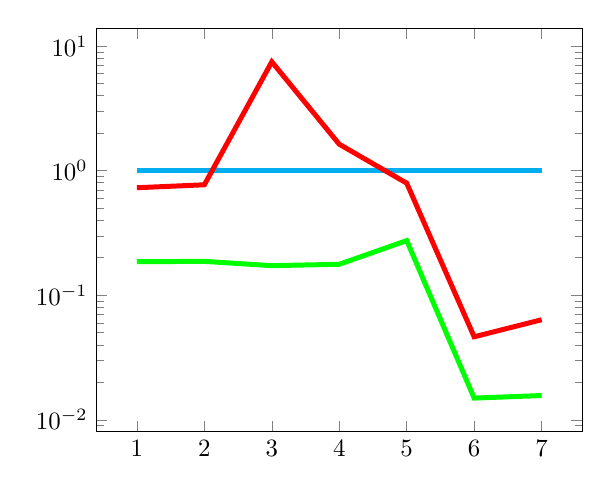
\begin{tikzpicture}[scale=0.9]
\begin{semilogyaxis}
\addplot[color=cyan,line width=2pt] coordinates {(1,1.0)(2,1.0)(3,1.0)(4,1.0)(5,1.0)(6,1.0)(7,1.0)};
\addplot[color=red,line width=2pt] coordinates {(1,0.7295664373818105)(2,0.7705529418912135)(3,7.478002658158148)(4,1.6306213479755793)(5,0.7939880646438021)(6,0.046389406927898606)(7,0.06359353530636197)};
\addplot[color=green,line width=2pt] coordinates {(1,0.18594867576897178)(2,0.1870324698038413)(3,0.17272803403737197)(4,0.17721928718854138)(5,0.2746859650255471)(6,0.014937936150121128)(7,0.01566247949178844)};

\end{semilogyaxis}
\end{tikzpicture}
